\documentclass[8pt]{article}
\usepackage[utf8]{inputenc}
% http://texdoc.net/texmf-dist/doc/latex/geometry/geometry.pdf
% https://mike42.me/blog/2016-01-how-to-arrange-pages-for-printing-and-cutting-in-latex

%Font
\usepackage[]{roboto} 

\renewcommand*\familydefault{\sfdefault} 	
\usepackage[T1]{fontenc}
%\usepackage{hyperref}

\usepackage{array}

\newcolumntype{x}[1]{%
>{\raggedleft\hspace{0pt}}p{#1}}%
% more font size definitions
\usepackage{moresize}	

\usepackage[paperwidth=90mm, paperheight=50mm, margin=3mm, showcrop=true]{geometry}
\usepackage{tikz}
\usetikzlibrary{shapes, backgrounds}

\usepackage{graphicx}
\usepackage{wrapfig}
\usepackage{ragged2e}

% use to vertically center content
% credits to: http://tex.stackexchange.com/questions/7219/how-to-vertically-center-two-images-next-to-each-other
\newcommand{\vcenteredinclude}[1]{\begingroup
\setbox0=\hbox{\includegraphics{#1}}%
\parbox{\wd0}{\box0}\endgroup}

% use to vertically center content
% credits to: http://tex.stackexchange.com/questions/7219/how-to-vertically-center-two-images-next-to-each-other
\newcommand*{\vcenteredhbox}[1]{\begingroup
\setbox0=\hbox{#1}\parbox{\wd0}{\box0}\endgroup}

% draw a circle with facts
% param 1: fact text
% param 2: scale default=1 (scales only chart, not label text)
% param 3: big border color
% param 4: second border color
% param 5: label bg color
\newcommand{\factbubble}[5]{
	\begin{tikzpicture}
	\pgfmathparse{#2*2}
	\let\pbxwidth\pgfmathresult
		\filldraw[fill=#3,draw=none] (0,0) circle (#2 * 1.5);
		\filldraw[fill=#5,draw=#4, line width=3.5pt] (0,0) circle (#2 * 1.2);
		\node at (0,0) {
			\parbox{\pbxwidth cm}{
				\begin{center}	
					#1
				\end{center}
			}
		};
	\end{tikzpicture}
}

\usepackage{color}
\definecolor{maincol}{HTML}{1B6D99}
\definecolor{secondcol}{HTML}{FCA311}
\definecolor{thirdcol}{HTML}{5CC8FF}
\definecolor{fourthcol}{HTML}{0B1F49}
\definecolor{fifthcol}{HTML}{eac381}
\definecolor{sixthcol}{RGB}{0,0,0}
\definecolor{textcol}{HTML}{000000}

%background color
\definecolor{bgcol}{HTML}{FFFFFF}%227,217,207}

%textcolor
%\definecolor{textcol}{HTML}{4B4E6D}

%sectioncolor
\definecolor{sectcol}{HTML}{FFFFFF}

%set a background col for whole page
\pagecolor{bgcol}

\usepackage{svg}
% SVG icons from https://www.svgrepo.com/
\newcommand{\icons}{svg/}	%path to your icon lib
\newcommand{\icon}[2]{\colorbox{secondcol}{\includesvg[height=#2, width=#2, distort=true]{\icons#1}}}	%icon shortcut
\newcommand{\icontext}[4]{ 						%icon with text shortcut
	\vcenteredhbox{\icon{#1}{#2}}\hspace{#4} \vcenteredhbox{\textcolor{textcol}{#3}}
	%\vcenteredhbox{\textcolor{textcol}{#3}} \hspace{5pt} \vcenteredhbox{\icon{#1}{#2}} \hspace{20pt}
}

\usepackage[cam,width=100truemm, height=60truemm,pdftex,center]{crop}
\begin{document}
\small
\hspace{-15pt}
\begin{minipage}{0.6\textwidth}
    \begin{flushleft}
\vspace{-5pt}
        \colorbox{maincol}{\large{\textcolor{white}{\textbf{\uppercase{Arianne Meijer}}} }}\\
            \hspace{0pt}
        \small{\textcolor{fourthcol}{\textsc{Pocket Resume}}}\\[10pt]
		\icontext{at}{10pt}{ariannemeijer@gmail.com}{5pt}\\[-2pt]
		\icontext{phone}{10pt}{+358 45 31 296 31}{5pt}\\[-2pt]
		\icontext{location}{10pt}{Espoo, Finland}{5pt}\\[-2pt]
		\icontext{linkedin}{10pt}{linkedin.com/in/aerylia}{5pt}
	\end{flushleft}
\end{minipage}
\begin{minipage}{0.4\textwidth}
	\begin{center}
        \colorbox{fourthcol}{\includegraphics[height=10pt]{\icons download}\hspace{14pt}\textcolor{white}{Full resume}\hspace{14pt}}\\
        %\hspace{15pt}
		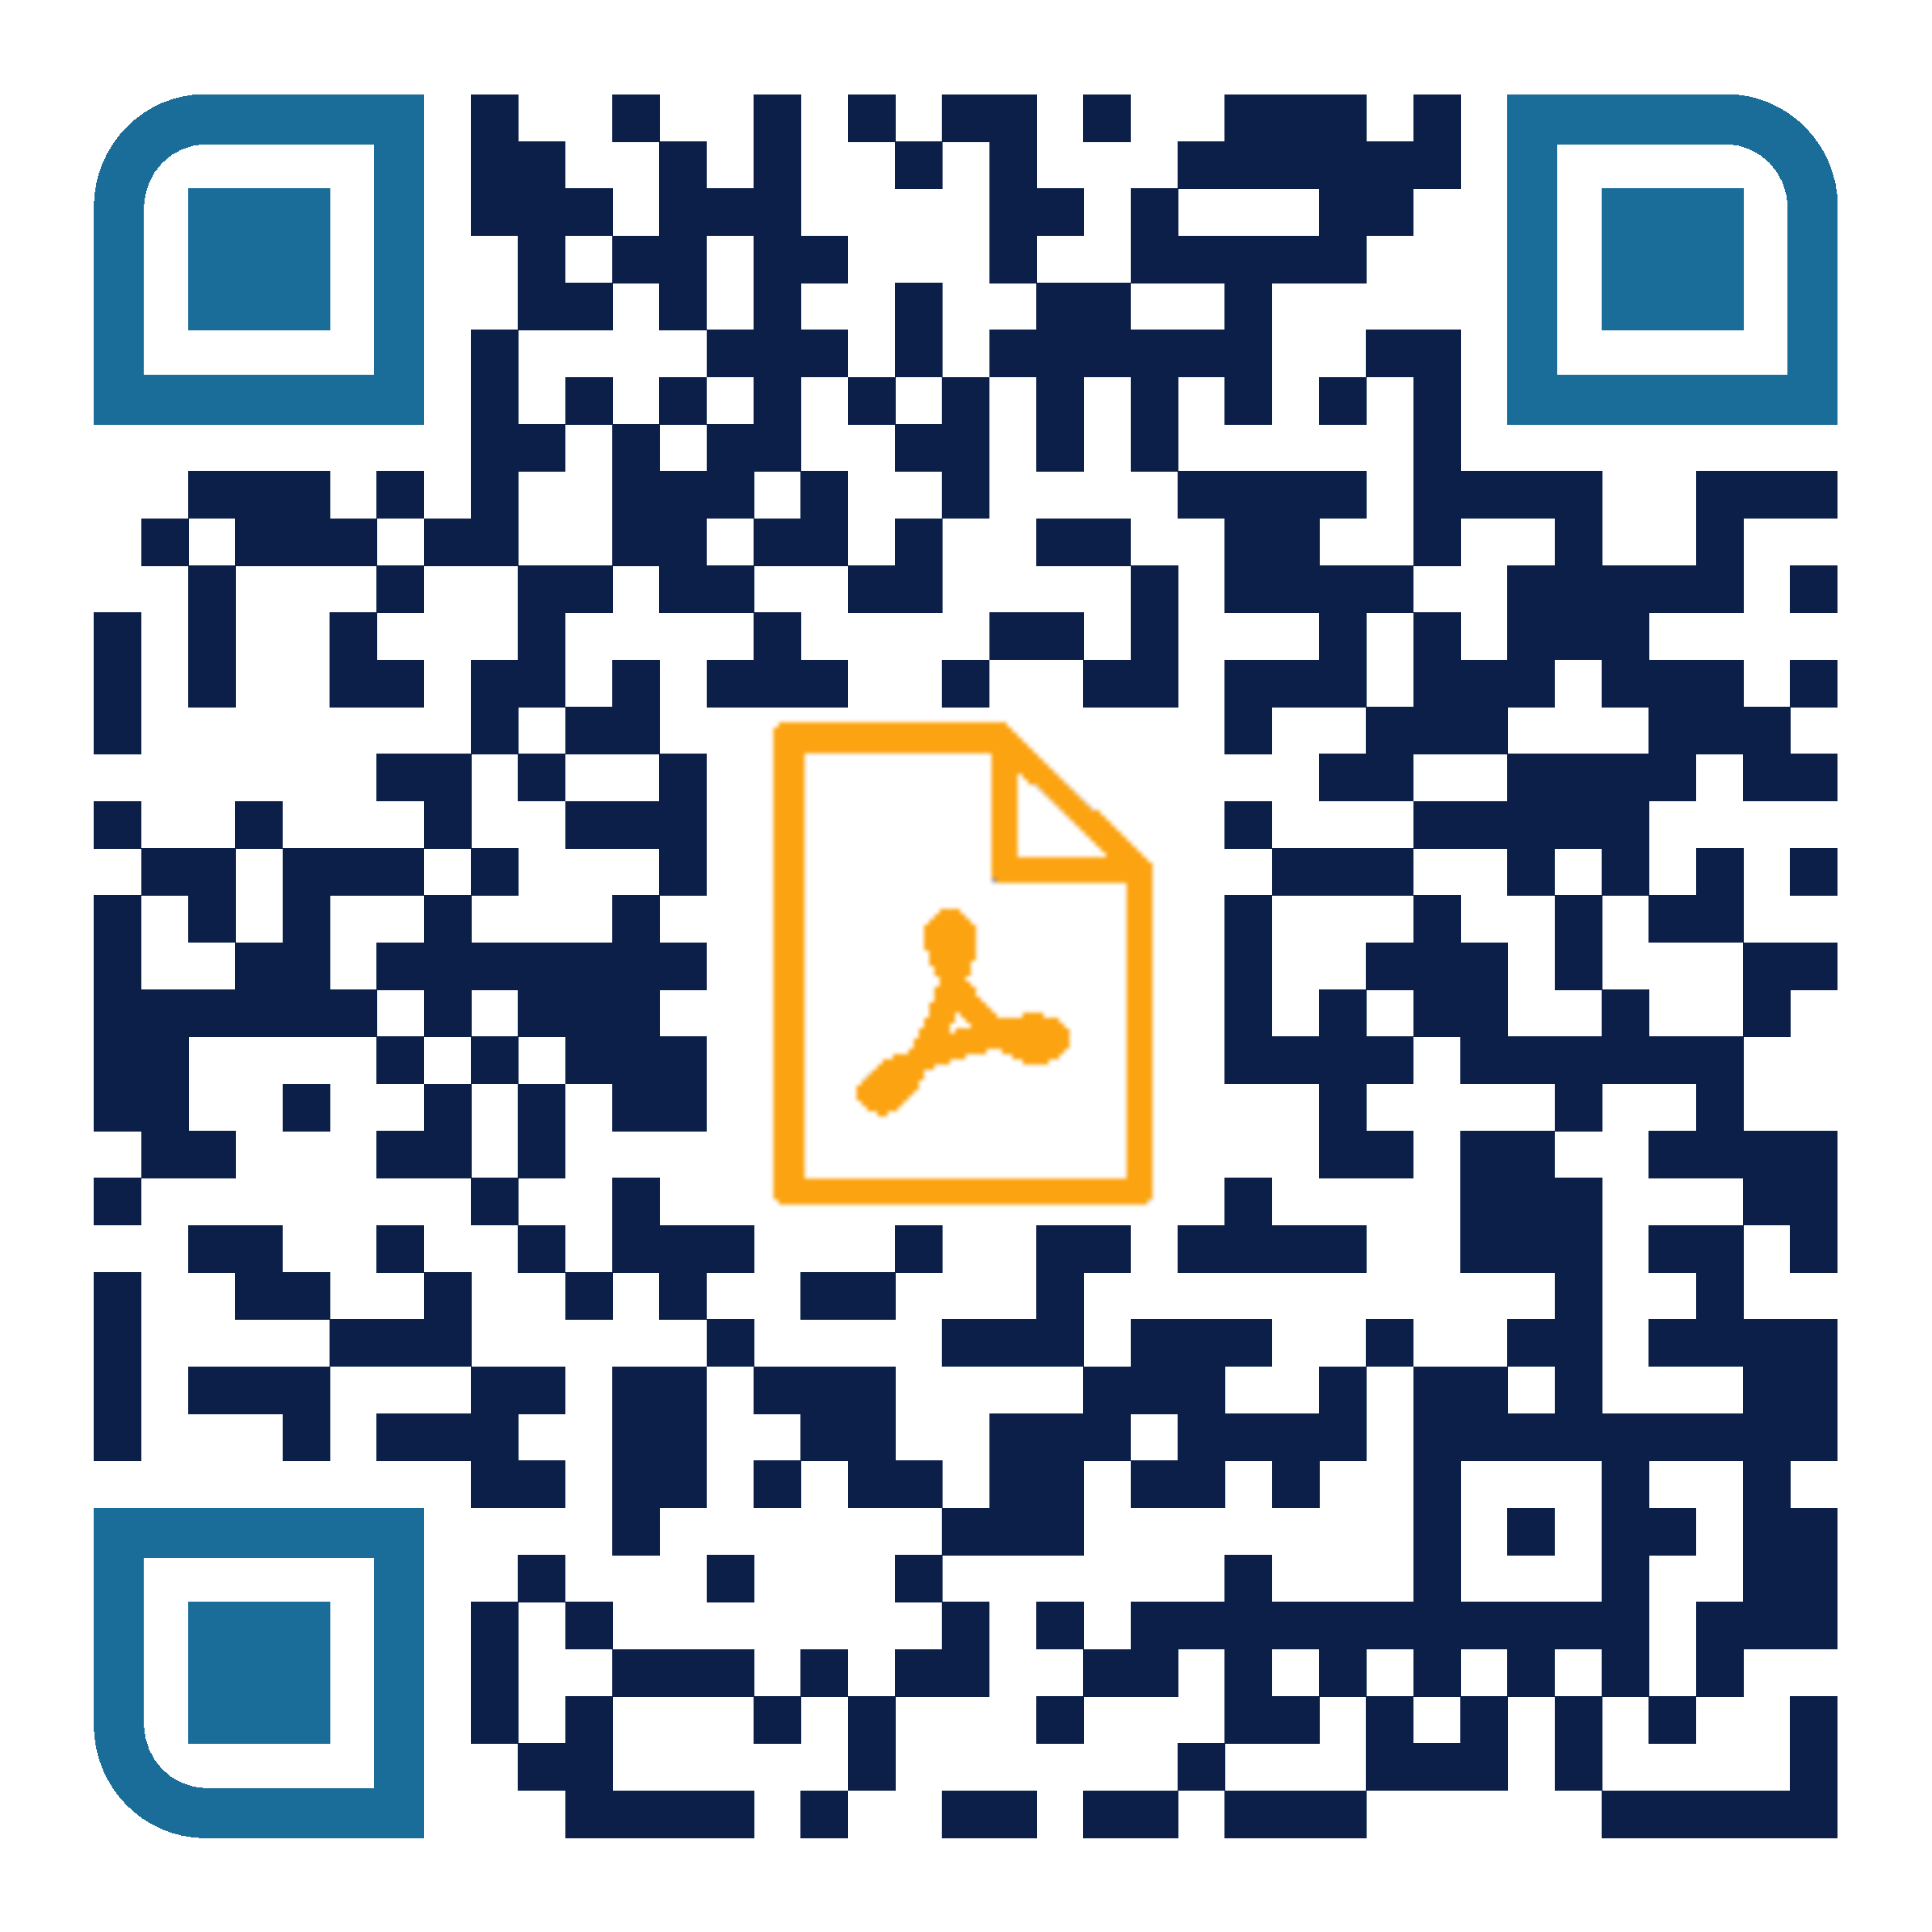
\includegraphics[width=0.9\textwidth]{qr-code2.pdf}
	\end{center}
\end{minipage}
\begin{center}
%\vspace{0pt}
\hspace{-6pt}
	\colorbox{thirdcol}{\hspace{15pt}\small{\textcolor{white}{\textbf{Computer Science PhD researcher, NISQ Software}}\hspace{9pt}}}
\end{center}
\newpage
        \begin{center}
            %\colorbox{maincol}{\large{\textcolor{white}{\textbf{T}}}\small{\textcolor{white}{oo}} \large{\textcolor{white}{\textbf{L}}}\small{\textcolor{white}{ong}} \large{\textcolor{white}{\textbf{; D}}}\small{\textcolor{white}{idn't}} \large{\textcolor{white}{\textbf{R}}}\small{\textcolor{white}{emember}}}\\
            \colorbox{maincol}{\textcolor{white}{\hspace{9pt}\uppercase{\textbf{Too long; Didn't Remember}}\hspace{9pt}}}
        \end{center}
        \ssmall
        \begin{flushleft}
            %\icontext{square-solid}{5pt}{\textcolor{fourthcol}{\textbf{Looking for an AI Master thesis project February - July 2019}}}{3pt}\\[2pt]
            \vspace{-5pt}
            \icontext{}{5pt}{\textcolor{fourthcol}{\textbf{Interested in fun and challenging problems to solve in new creative ways}}}{3pt}\\[1pt]
            \icontext{}{5pt}{\textcolor{fourthcol}{\textbf{Languages:}} Dutch (native), English (professional), German (intermediate)}{3pt}\\[1pt]
            \icontext{}{5pt}{\textcolor{fourthcol}{\textbf{Languages:}} Python (main), Java (advanced), C (basic), Haskell/Clean (basic)}{3pt}\\[1pt]
            \icontext{}{5pt}{\textcolor{fourthcol}{\textbf{Worked at:}} Cambridge Quantum (now Quantinuum), Atos, RadboudUMC}{3pt}\\[1pt]
            \icontext{}{5pt}{\textcolor{fourthcol}{\textbf{Interests:}} Quantum Computing, Machine Learning, Natural Language Processing}{3pt}\\[1pt]
            \icontext{}{5pt}{\textcolor{fourthcol}{\textbf{Hobbies:}} Knitting, Swimming, Logic puzzles, Anime, Miniature painting, Singing}{3pt}\\[1pt]
            \icontext{}{5pt}{\textcolor{fourthcol}{\textbf{Obtained degrees:}} Msc. Computer Science \& Artificial Intelligence (cum laude)}{3pt}\\[1pt]
            \icontext{}{5pt}{\textcolor{fourthcol}{\textbf{Expected graduation:}} Summer 2023, CS PhD student}{3pt}\\[1pt]
            \icontext{}{5pt}{\textcolor{fourthcol}{\textbf{Resume in QR code will stay up-to-date}} }{3pt}
        \end{flushleft}
        \begin{flushright}
            \vspace{-25pt}
            \hspace{-2pt}
            ORCID ID:\\
            \hspace{-2pt}
			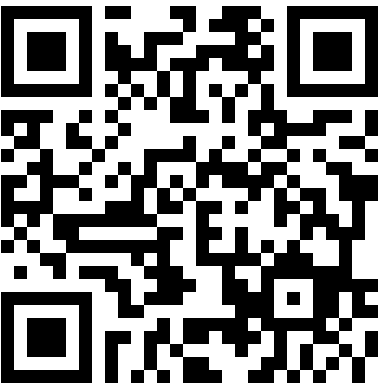
\includegraphics[height=45pt]{ORCID_QR_code.png}
        \end{flushright}
            \vspace{-26pt}
			\colorbox{thirdcol}{\hspace{9pt}\small{\textcolor{white}{\textbf{University of Helsinki}}\hspace{9pt}}}
\end{document}
